\section{Complete Canonical Numerical Records}
\label{sec:supp-canonical-records}

This section collects the full numerical records referenced by the main
paper's Appendix~D.  The tables below are typeset directly from the committed
CSV files; compilation does not rerun either numerical solver.  Exact rational
fields retain their machine-readable \texttt{numerator//denominator} form.
The compact stationary table is duplicated from the main paper to make the
record self-contained.

\newcommand{\recordfield}[1]{{\ttfamily\expandafter\detokenize\expandafter{#1}}}

\clearpage
\subsection{Convergence history and stationary solution}

\begin{figure}[htbp]
  \centering
  % Generated by julia/scripts/generate_manuscript_numerical_artifacts.jl.
% Source: experiments/results/summaries/unified_canonical_convergence.csv.
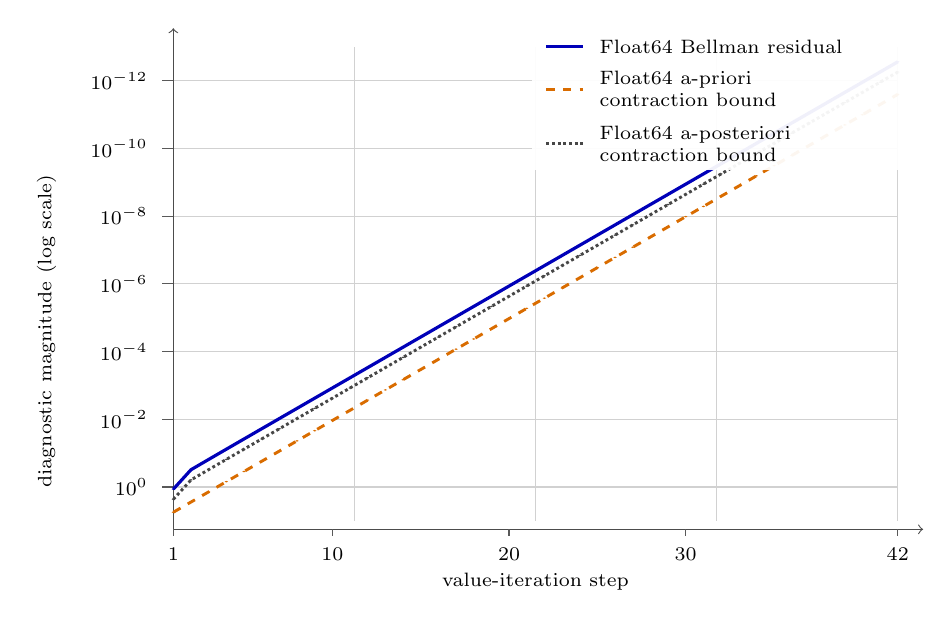
\begin{tikzpicture}[x=0.92cm,y=0.43cm,font=\scriptsize]
  \draw[black!18] (0,-1) grid[xstep=2.5,ystep=2] (10,13);
  \draw[->,black!70] (0,-1.25) -- (10.35,-1.25);
  \draw[->,black!70] (0,-1.25) -- (0,13.55);
  \foreach \x/\label in {0/1,2.195/10,4.634/20,7.073/30,10/42} {
    \draw[black!65] (\x,-1.25) -- (\x,-1.45);
    \node[anchor=north] at (\x,-1.5) {\label};
  }
  \foreach \y/\label in {0/{$10^{0}$},2/{$10^{-2}$},4/{$10^{-4}$},6/{$10^{-6}$},8/{$10^{-8}$},10/{$10^{-10}$},12/{$10^{-12}$}} {
    \draw[black!65] (0,\y) -- (-0.16,\y);
    \node[anchor=east] at (-0.22,\y) {\label};
  }
  \draw[blue!72!black,line width=1.15pt] (0.0,-0.063052) -- (0.243902,0.510613) -- (0.487805,0.8144) -- (0.731707,1.116816) -- (0.97561,1.41854) -- (1.219512,1.719917) -- (1.463415,2.021121) -- (1.707317,2.322238) -- (1.95122,2.623312) -- (2.195122,2.924364) -- (2.439024,3.225404) -- (2.682927,3.52644) -- (2.926829,3.827473) -- (3.170732,4.128504) -- (3.414634,4.429535) -- (3.658537,4.730565) -- (3.902439,5.031595) -- (4.146341,5.332625) -- (4.390244,5.633655) -- (4.634146,5.934685) -- (4.878049,6.235715) -- (5.121951,6.536745) -- (5.365854,6.837775) -- (5.609756,7.138805) -- (5.853659,7.439835) -- (6.097561,7.740865) -- (6.341463,8.041895) -- (6.585366,8.342925) -- (6.829268,8.643955) -- (7.073171,8.944985) -- (7.317073,9.246015) -- (7.560976,9.547045) -- (7.804878,9.848075) -- (8.04878,10.149105) -- (8.292683,10.450135) -- (8.536585,10.751165) -- (8.780488,11.052195) -- (9.02439,11.353225) -- (9.268293,11.654255) -- (9.512195,11.955285) -- (9.756098,12.256315) -- (10.0,12.557345);
  \draw[orange!85!black,line width=1.05pt,dashed] (0.0,-0.74527) -- (0.243902,-0.44424) -- (0.487805,-0.14321) -- (0.731707,0.15782) -- (0.97561,0.45885) -- (1.219512,0.75988) -- (1.463415,1.06091) -- (1.707317,1.36194) -- (1.95122,1.66297) -- (2.195122,1.964) -- (2.439024,2.26503) -- (2.682927,2.56606) -- (2.926829,2.86709) -- (3.170732,3.16812) -- (3.414634,3.46915) -- (3.658537,3.77018) -- (3.902439,4.07121) -- (4.146341,4.37224) -- (4.390244,4.67327) -- (4.634146,4.9743) -- (4.878049,5.27533) -- (5.121951,5.57636) -- (5.365854,5.87739) -- (5.609756,6.17842) -- (5.853659,6.47945) -- (6.097561,6.78048) -- (6.341463,7.08151) -- (6.585366,7.38254) -- (6.829268,7.68357) -- (7.073171,7.9846) -- (7.317073,8.28563) -- (7.560976,8.58666) -- (7.804878,8.88769) -- (8.04878,9.18872) -- (8.292683,9.48975) -- (8.536585,9.79078) -- (8.780488,10.09181) -- (9.02439,10.39284) -- (9.268293,10.69387) -- (9.512195,10.9949) -- (9.756098,11.29593) -- (10.0,11.59696);
  \draw[black!72,line width=1.05pt,densely dotted] (0.0,-0.364082) -- (0.243902,0.209583) -- (0.487805,0.51337) -- (0.731707,0.815786) -- (0.97561,1.11751) -- (1.219512,1.418887) -- (1.463415,1.720091) -- (1.707317,2.021208) -- (1.95122,2.322282) -- (2.195122,2.623334) -- (2.439024,2.924374) -- (2.682927,3.22541) -- (2.926829,3.526443) -- (3.170732,3.827474) -- (3.414634,4.128505) -- (3.658537,4.429535) -- (3.902439,4.730565) -- (4.146341,5.031595) -- (4.390244,5.332625) -- (4.634146,5.633655) -- (4.878049,5.934685) -- (5.121951,6.235715) -- (5.365854,6.536745) -- (5.609756,6.837775) -- (5.853659,7.138805) -- (6.097561,7.439835) -- (6.341463,7.740865) -- (6.585366,8.041895) -- (6.829268,8.342925) -- (7.073171,8.643955) -- (7.317073,8.944985) -- (7.560976,9.246015) -- (7.804878,9.547045) -- (8.04878,9.848075) -- (8.292683,10.149105) -- (8.536585,10.450135) -- (8.780488,10.751165) -- (9.02439,11.052195) -- (9.268293,11.353225) -- (9.512195,11.654255) -- (9.756098,11.955285) -- (10.0,12.256315);
  \fill[blue!72!black] (0.0,-0.063052) circle (0.024);
  \fill[blue!72!black] (0.243902,0.510613) circle (0.024);
  \fill[blue!72!black] (0.487805,0.8144) circle (0.024);
  \fill[blue!72!black] (0.731707,1.116816) circle (0.024);
  \fill[blue!72!black] (0.97561,1.41854) circle (0.024);
  \fill[blue!72!black] (1.219512,1.719917) circle (0.024);
  \fill[blue!72!black] (1.463415,2.021121) circle (0.024);
  \fill[blue!72!black] (1.707317,2.322238) circle (0.024);
  \fill[blue!72!black] (1.95122,2.623312) circle (0.024);
  \fill[blue!72!black] (2.195122,2.924364) circle (0.024);
  \fill[blue!72!black] (2.439024,3.225404) circle (0.024);
  \fill[blue!72!black] (2.682927,3.52644) circle (0.024);
  \fill[blue!72!black] (2.926829,3.827473) circle (0.024);
  \fill[blue!72!black] (3.170732,4.128504) circle (0.024);
  \fill[blue!72!black] (3.414634,4.429535) circle (0.024);
  \fill[blue!72!black] (3.658537,4.730565) circle (0.024);
  \fill[blue!72!black] (3.902439,5.031595) circle (0.024);
  \fill[blue!72!black] (4.146341,5.332625) circle (0.024);
  \fill[blue!72!black] (4.390244,5.633655) circle (0.024);
  \fill[blue!72!black] (4.634146,5.934685) circle (0.024);
  \fill[blue!72!black] (4.878049,6.235715) circle (0.024);
  \fill[blue!72!black] (5.121951,6.536745) circle (0.024);
  \fill[blue!72!black] (5.365854,6.837775) circle (0.024);
  \fill[blue!72!black] (5.609756,7.138805) circle (0.024);
  \fill[blue!72!black] (5.853659,7.439835) circle (0.024);
  \fill[blue!72!black] (6.097561,7.740865) circle (0.024);
  \fill[blue!72!black] (6.341463,8.041895) circle (0.024);
  \fill[blue!72!black] (6.585366,8.342925) circle (0.024);
  \fill[blue!72!black] (6.829268,8.643955) circle (0.024);
  \fill[blue!72!black] (7.073171,8.944985) circle (0.024);
  \fill[blue!72!black] (7.317073,9.246015) circle (0.024);
  \fill[blue!72!black] (7.560976,9.547045) circle (0.024);
  \fill[blue!72!black] (7.804878,9.848075) circle (0.024);
  \fill[blue!72!black] (8.04878,10.149105) circle (0.024);
  \fill[blue!72!black] (8.292683,10.450135) circle (0.024);
  \fill[blue!72!black] (8.536585,10.751165) circle (0.024);
  \fill[blue!72!black] (8.780488,11.052195) circle (0.024);
  \fill[blue!72!black] (9.02439,11.353225) circle (0.024);
  \fill[blue!72!black] (9.268293,11.654255) circle (0.024);
  \fill[blue!72!black] (9.512195,11.955285) circle (0.024);
  \fill[blue!72!black] (9.756098,12.256315) circle (0.024);
  \fill[blue!72!black] (10.0,12.557345) circle (0.024);
  \fill[orange!85!black] (0.0,-0.74527) circle (0.024);
  \fill[orange!85!black] (0.243902,-0.44424) circle (0.024);
  \fill[orange!85!black] (0.487805,-0.14321) circle (0.024);
  \fill[orange!85!black] (0.731707,0.15782) circle (0.024);
  \fill[orange!85!black] (0.97561,0.45885) circle (0.024);
  \fill[orange!85!black] (1.219512,0.75988) circle (0.024);
  \fill[orange!85!black] (1.463415,1.06091) circle (0.024);
  \fill[orange!85!black] (1.707317,1.36194) circle (0.024);
  \fill[orange!85!black] (1.95122,1.66297) circle (0.024);
  \fill[orange!85!black] (2.195122,1.964) circle (0.024);
  \fill[orange!85!black] (2.439024,2.26503) circle (0.024);
  \fill[orange!85!black] (2.682927,2.56606) circle (0.024);
  \fill[orange!85!black] (2.926829,2.86709) circle (0.024);
  \fill[orange!85!black] (3.170732,3.16812) circle (0.024);
  \fill[orange!85!black] (3.414634,3.46915) circle (0.024);
  \fill[orange!85!black] (3.658537,3.77018) circle (0.024);
  \fill[orange!85!black] (3.902439,4.07121) circle (0.024);
  \fill[orange!85!black] (4.146341,4.37224) circle (0.024);
  \fill[orange!85!black] (4.390244,4.67327) circle (0.024);
  \fill[orange!85!black] (4.634146,4.9743) circle (0.024);
  \fill[orange!85!black] (4.878049,5.27533) circle (0.024);
  \fill[orange!85!black] (5.121951,5.57636) circle (0.024);
  \fill[orange!85!black] (5.365854,5.87739) circle (0.024);
  \fill[orange!85!black] (5.609756,6.17842) circle (0.024);
  \fill[orange!85!black] (5.853659,6.47945) circle (0.024);
  \fill[orange!85!black] (6.097561,6.78048) circle (0.024);
  \fill[orange!85!black] (6.341463,7.08151) circle (0.024);
  \fill[orange!85!black] (6.585366,7.38254) circle (0.024);
  \fill[orange!85!black] (6.829268,7.68357) circle (0.024);
  \fill[orange!85!black] (7.073171,7.9846) circle (0.024);
  \fill[orange!85!black] (7.317073,8.28563) circle (0.024);
  \fill[orange!85!black] (7.560976,8.58666) circle (0.024);
  \fill[orange!85!black] (7.804878,8.88769) circle (0.024);
  \fill[orange!85!black] (8.04878,9.18872) circle (0.024);
  \fill[orange!85!black] (8.292683,9.48975) circle (0.024);
  \fill[orange!85!black] (8.536585,9.79078) circle (0.024);
  \fill[orange!85!black] (8.780488,10.09181) circle (0.024);
  \fill[orange!85!black] (9.02439,10.39284) circle (0.024);
  \fill[orange!85!black] (9.268293,10.69387) circle (0.024);
  \fill[orange!85!black] (9.512195,10.9949) circle (0.024);
  \fill[orange!85!black] (9.756098,11.29593) circle (0.024);
  \fill[orange!85!black] (10.0,11.59696) circle (0.024);
  \fill[black!72] (0.0,-0.364082) circle (0.024);
  \fill[black!72] (0.243902,0.209583) circle (0.024);
  \fill[black!72] (0.487805,0.51337) circle (0.024);
  \fill[black!72] (0.731707,0.815786) circle (0.024);
  \fill[black!72] (0.97561,1.11751) circle (0.024);
  \fill[black!72] (1.219512,1.418887) circle (0.024);
  \fill[black!72] (1.463415,1.720091) circle (0.024);
  \fill[black!72] (1.707317,2.021208) circle (0.024);
  \fill[black!72] (1.95122,2.322282) circle (0.024);
  \fill[black!72] (2.195122,2.623334) circle (0.024);
  \fill[black!72] (2.439024,2.924374) circle (0.024);
  \fill[black!72] (2.682927,3.22541) circle (0.024);
  \fill[black!72] (2.926829,3.526443) circle (0.024);
  \fill[black!72] (3.170732,3.827474) circle (0.024);
  \fill[black!72] (3.414634,4.128505) circle (0.024);
  \fill[black!72] (3.658537,4.429535) circle (0.024);
  \fill[black!72] (3.902439,4.730565) circle (0.024);
  \fill[black!72] (4.146341,5.031595) circle (0.024);
  \fill[black!72] (4.390244,5.332625) circle (0.024);
  \fill[black!72] (4.634146,5.633655) circle (0.024);
  \fill[black!72] (4.878049,5.934685) circle (0.024);
  \fill[black!72] (5.121951,6.235715) circle (0.024);
  \fill[black!72] (5.365854,6.536745) circle (0.024);
  \fill[black!72] (5.609756,6.837775) circle (0.024);
  \fill[black!72] (5.853659,7.138805) circle (0.024);
  \fill[black!72] (6.097561,7.439835) circle (0.024);
  \fill[black!72] (6.341463,7.740865) circle (0.024);
  \fill[black!72] (6.585366,8.041895) circle (0.024);
  \fill[black!72] (6.829268,8.342925) circle (0.024);
  \fill[black!72] (7.073171,8.643955) circle (0.024);
  \fill[black!72] (7.317073,8.944985) circle (0.024);
  \fill[black!72] (7.560976,9.246015) circle (0.024);
  \fill[black!72] (7.804878,9.547045) circle (0.024);
  \fill[black!72] (8.04878,9.848075) circle (0.024);
  \fill[black!72] (8.292683,10.149105) circle (0.024);
  \fill[black!72] (8.536585,10.450135) circle (0.024);
  \fill[black!72] (8.780488,10.751165) circle (0.024);
  \fill[black!72] (9.02439,11.052195) circle (0.024);
  \fill[black!72] (9.268293,11.353225) circle (0.024);
  \fill[black!72] (9.512195,11.654255) circle (0.024);
  \fill[black!72] (9.756098,11.955285) circle (0.024);
  \fill[black!72] (10.0,12.256315) circle (0.024);
  \fill[white,opacity=0.94] (4.95,9.35) rectangle (10.15,13.45);
  \draw[blue!72!black,line width=1.15pt] (5.15,13.0) -- (5.65,13.0);
  \node[anchor=west] at (5.75,13.0) {Float64 Bellman residual};
  \draw[orange!85!black,line width=1.05pt,dashed] (5.15,11.75) -- (5.65,11.75);
  \node[anchor=west,align=left] at (5.75,11.75) {Float64 a-priori\\contraction bound};
  \draw[black!72,line width=1.05pt,densely dotted] (5.15,10.15) -- (5.65,10.15);
  \node[anchor=west,align=left] at (5.75,10.15) {Float64 a-posteriori\\contraction bound};
  \node[anchor=north] at (5,-2.25) {value-iteration step};
  \node[rotate=90] at (-1.75,4.6) {diagnostic magnitude (log scale)};
\end{tikzpicture}

  \caption{Complete Float64 convergence history for the unified six-state
  benchmark.  Markers are the 42 committed iterations; joining segments are
  visual guides.  The dotted series is the Float64 a-posteriori contraction
  bound.  Exact rational policy iteration is a separate calculation with
  Bellman residual zero.}
  \label{fig:supp-canonical-convergence}
\end{figure}

The final convergence-row bound is
\(r_{42}^{64}/(1-\beta_{64})=5.54223\times10^{-13}\), computed in Float64.
The canonical summary separately converts the binary iterate exactly to
\texttt{Rational\{BigInt\}}, records maximum exact error
\(937/1688849860263936\approx5.5482\times10^{-13}\), and evaluates the exact
rational Bellman residual to obtain the exactly re-evaluated residual-based
certificate
\(2499/4503599627370496\approx5.5489\times10^{-13}\).  The latter is not the
residual-bound column in the convergence table.

\begin{landscape}
\scriptsize
\csvreader[
  longtable={@{}rllll@{}},
  table head={\caption{Full 42-row Float64 convergence record.}
    \label{tab:supp-convergence-history}\\
    \toprule
    Iter. & Float64 increment & Float64 Bellman residual &
    \shortstack{Float64 a-priori\\contraction bound} &
    \shortstack{Float64 a-posteriori\\contraction bound}\\
    \midrule\endfirsthead
    \toprule
    Iter. & Float64 increment & Float64 Bellman residual &
    \shortstack{Float64 a-priori\\contraction bound} &
    \shortstack{Float64 a-posteriori\\contraction bound}\\
    \midrule\endhead
    \bottomrule\endfoot}
]{data/unified_canonical_convergence.csv}{
  iteration=\iteration,
  float64_iteration_increment=\increment,
  float64_bellman_residual=\bellmanresidual,
  float64_apriori_contraction_bound=\aprioribound,
  float64_aposteriori_contraction_bound=\residualbound
}{\recordfield{\iteration} & \recordfield{\increment} &
  \recordfield{\bellmanresidual} & \recordfield{\aprioribound} &
  \recordfield{\residualbound}}
\end{landscape}

\setlength{\tabcolsep}{1pt}
\begin{landscape}
\begin{center}
\small
% Generated by julia/scripts/generate_main_text_tables.jl.
% Exact source: experiments/results/summaries/unified_canonical_resource_channel_elasticities.csv.
\begin{tabular}{@{}llrll@{}}
\toprule
State & Belief & \(V^\star\) (payoff units) & \(\pi^\star\) & Winning margin (payoff units) \\
\midrule
\(K_{0}\)&\(\ell\)&\(\frac{115}{288}\)&Discover&\(\frac{23}{96}\)\\
\(K_{0}\)&\(h\)&\(\frac{23}{288}\)&Continue&\(\frac{245}{384}\)\\
\(K_{1}\)&\(\ell\)&\(1\)&Scale&\(\frac{23}{48}\)\\
\(K_{1}\)&\(h\)&\(\frac{7}{6}\)&Scale&\(\frac{29}{48}\)\\
\(K_{2}\)&\(\ell\)&\(\frac{14}{3}\)&Continue&\(\frac{3}{16}\)\\
\(K_{2}\)&\(h\)&\(\frac{22}{3}\)&Continue&\(\frac{3}{16}\)\\
\bottomrule
\end{tabular}

\refstepcounter{table}\label{tab:supp-stationary-solution}

\smallskip
Table~\thetable: Exact rational stationary solution, duplicated from the main
paper.
\end{center}

\tiny
\csvreader[
  longtable={@{}lllllllrrrrr@{}},
  table head={\caption{Complete stationary action-value record.}
    \label{tab:supp-action-values}\\
    \toprule
    State & Belief & Value & Chosen & Second & Continue (Q) & Research &
    Research (Q) & Margin & Duration & Reward block & Discounted continuation\\
    \midrule\endfirsthead
    \toprule
    State & Belief & Value & Chosen & Second & Continue (Q) & Research &
    Research (Q) & Margin & Duration & Reward block & Discounted continuation\\
    \midrule\endhead
    \bottomrule\endfoot}
]{data/unified_benchmark_policy_value.csv}{
  compressed_state=\state,
  belief=\belief,
  value=\stationaryvalue,
  chosen_action=\chosen,
  second_action=\second,
  continue_q=\continueq,
  research_action=\research,
  research_q=\researchq,
  action_margin=\margin,
  project_duration=\duration,
  expected_project_reward_block=\rewardblock,
  discounted_project_continuation=\continuationblock
}{\recordfield{\state} & \recordfield{\belief} & \recordfield{\stationaryvalue} &
  \recordfield{\chosen} & \recordfield{\second} & \recordfield{\continueq} &
  \recordfield{\research} & \recordfield{\researchq} &
  \recordfield{\margin} & \recordfield{\duration} &
  \recordfield{\rewardblock} & \recordfield{\continuationblock}}
\end{landscape}

\setlength{\tabcolsep}{2pt}
\begin{landscape}
\subsection{Horizon-by-horizon values and actions}

The value record includes horizons zero through eight and all four stationary
solution/evaluation outputs.  The policy record includes every positive
finite horizon and both stationary policy outputs.  This retains the exact
and floating-point rows together rather than presenting a selectively rounded
comparison.

\scriptsize
\csvreader[
  longtable={@{}p{0.27\linewidth}p{0.06\linewidth}p{0.16\linewidth}p{0.08\linewidth}p{0.08\linewidth}p{0.27\linewidth}@{}},
  table head={\caption{Complete horizon-by-horizon and stationary value record.}
    \label{tab:supp-horizon-values}\\
    \toprule
    Solution & Horizon & Arithmetic & State & Belief & Value\\
    \midrule\endfirsthead
    \toprule
    Solution & Horizon & Arithmetic & State & Belief & Value\\
    \midrule\endhead
    \bottomrule\endfoot}
]{data/unified_canonical_values.csv}{
  solution=\solution,
  horizon=\horizon,
  arithmetic=\arithmetic,
  compressed_state=\state,
  belief=\belief,
  value=\recordvalue
}{\recordfield{\solution} & \recordfield{\horizon} &
  \recordfield{\arithmetic} & \recordfield{\state} &
  \recordfield{\belief} & \recordfield{\recordvalue}}
\end{landscape}

\begin{landscape}
\scriptsize
\csvreader[
  longtable={@{}p{0.34\linewidth}p{0.08\linewidth}p{0.12\linewidth}p{0.12\linewidth}p{0.25\linewidth}@{}},
  table head={\caption{Complete horizon-by-horizon and stationary action record.}
    \label{tab:supp-horizon-actions}\\
    \toprule
    Solution & Horizon & State & Belief & Action\\
    \midrule\endfirsthead
    \toprule
    Solution & Horizon & State & Belief & Action\\
    \midrule\endhead
    \bottomrule\endfoot}
]{data/unified_canonical_policies.csv}{
  solution=\solution,
  horizon=\horizon,
  compressed_state=\state,
  belief=\belief,
  action=\action
}{\recordfield{\solution} & \recordfield{\horizon} &
  \recordfield{\state} & \recordfield{\belief} & \recordfield{\action}}
\end{landscape}

\begin{landscape}
\subsection{Path, admission, and operating-reward atoms}

\tiny
\csvreader[
  longtable={@{}llllllllll@{}},
  table head={\caption{Complete positive-duration path and admission-atom record.}
    \label{tab:supp-path-admission-atoms}\\
    \toprule
    Project & Start state & Start belief & Duration & Path & Terminal belief &
    Admitted & Joint mass & Path mass & Conditional admission\\
    \midrule\endfirsthead
    \toprule
    Project & Start state & Start belief & Duration & Path & Terminal belief &
    Admitted & Joint mass & Path mass & Conditional admission\\
    \midrule\endhead
    \bottomrule\endfoot}
]{data/unified_canonical_duration_paths.csv}{
  project=\project,
  start_state=\startstate,
  start_belief=\startbelief,
  duration=\duration,
  path=\beliefpath,
  terminal_belief=\terminalbelief,
  admitted=\admitted,
  joint_mass=\jointmass,
  path_mass=\pathmass,
  conditional_admission_mass=\conditionalmass
}{\recordfield{\project} & \recordfield{\startstate} &
  \recordfield{\startbelief} & \recordfield{\duration} &
  \recordfield{\beliefpath} & \recordfield{\terminalbelief} &
  \recordfield{\admitted} & \recordfield{\jointmass} &
  \recordfield{\pathmass} & \recordfield{\conditionalmass}}

\tiny
\csvreader[
  longtable={@{}llllllll@{}},
  table head={\caption{Complete operating-reward block record.}
    \label{tab:supp-operating-rewards}\\
    \toprule
    State & Belief & Action & Duration & Operates & Initiation cost &
    Incumbent reward & Net reward block\\
    \midrule\endfirsthead
    \toprule
    State & Belief & Action & Duration & Operates & Initiation cost &
    Incumbent reward & Net reward block\\
    \midrule\endhead
    \bottomrule\endfoot}
]{data/unified_canonical_operating_rewards.csv}{
  compressed_state=\state,
  belief=\belief,
  action=\action,
  duration=\duration,
  operates_during_research=\operates,
  initiation_cost=\cost,
  expected_incumbent_reward=\incumbentreward,
  expected_net_reward_block=\netreward
}{\recordfield{\state} & \recordfield{\belief} & \recordfield{\action} &
  \recordfield{\duration} & \recordfield{\operates} & \recordfield{\cost} &
  \recordfield{\incumbentreward} & \recordfield{\netreward}}
\end{landscape}

\begin{landscape}
\subsection{Safe compression and capacity correspondences}

The following tables retain every source and every optimizer tie.  Masks use
the coordinate order \((I,A,B,D)\); semicolon-separated entries are tied
solutions, not a sequence of selections.
The primary burden keeps \(w_I=w_{s_0}=0\).  The committed canonical resource
artifacts use the separately displayed total
\(\widetilde W(L)=1+W(L)\), so their machine fields
\texttt{source\_burden}, \texttt{capacity}, \texttt{optimal\_burdens}, and
\texttt{selected\_burden} are display burdens.  Consequently the capacity
objective is \(\widetilde V^\star(b;\widetilde B)\) and the penalized net-value
field is \(\widetilde J^\star(b;\lambda)=J^\star(b;\lambda)-\lambda\).
Absolute burden reductions and all switching prices are invariant to this
common-unit translation.  The capacity theorem and Lean formalization use
\(W\), not \(\widetilde W\).

\tiny
\csvreader[
  longtable={@{}llllllllllll@{}},
  table head={\caption{Complete safe-compression optimizer correspondence.}
    \label{tab:supp-safe-compression}\\
    \toprule
    Schedule & Source mask & Source library & \shortstack{Display source\\burden \(\widetilde W\)} & Feasible masks & \shortstack{Minimum display\\burden \(\widetilde W\)} &
    Optimal masks & Optimal libraries & \shortstack{Burden reduction\\\(\Delta\widetilde W=\Delta W\)} & Frontier & Closure & Ties complete\\
    \midrule\endfirsthead
    \toprule
    Schedule & Source mask & Source library & \shortstack{Display source\\burden \(\widetilde W\)} & Feasible masks & \shortstack{Minimum display\\burden \(\widetilde W\)} &
    Optimal masks & Optimal libraries & \shortstack{Burden reduction\\\(\Delta\widetilde W=\Delta W\)} & Frontier & Closure & Ties complete\\
    \midrule\endhead
    \bottomrule\endfoot}
]{data/unified_canonical_resource_safe_compression.csv}{
  schedule=\schedule,
  source_mask=\sourcemask,
  source_library=\sourcelibrary,
  source_burden=\sourceburden,
  feasible_masks=\feasiblemasks,
  optimal_objective=\objective,
  optimal_masks=\optimalmasks,
  optimal_libraries=\optimallibraries,
  burden_reduction=\reduction,
  frontier=\frontier,
  closure=\closure,
  ties_complete=\tiescomplete
}{\recordfield{\schedule} & \recordfield{\sourcemask} &
  \recordfield{\sourcelibrary} & \recordfield{\sourceburden} &
  \recordfield{\feasiblemasks} & \recordfield{\objective} &
  \recordfield{\optimalmasks} & \recordfield{\optimallibraries} &
  \recordfield{\reduction} & \recordfield{\frontier} &
  \recordfield{\closure} & \recordfield{\tiescomplete}}

\newpage
\tiny
\csvreader[
  longtable={@{}llllllllllll@{}},
  table head={\caption{Complete capacity paths and value certificates.}
    \label{tab:supp-capacity-paths}\\
    \toprule
    Schedule & Belief & \shortstack{Display capacity\\\(\widetilde B\)} & \(\widetilde V^\star\) & Optimal masks & Optimal libraries &
    \shortstack{Optimal display\\burdens \(\widetilde W\)} & Selected library & Op. value & Gen. value & Total value & Ties complete\\
    \midrule\endfirsthead
    \toprule
    Schedule & Belief & \shortstack{Display capacity\\\(\widetilde B\)} & \(\widetilde V^\star\) & Optimal masks & Optimal libraries &
    \shortstack{Optimal display\\burdens \(\widetilde W\)} & Selected library & Op. value & Gen. value & Total value & Ties complete\\
    \midrule\endhead
    \bottomrule\endfoot}
]{data/unified_canonical_resource_capacity.csv}{
  schedule=\schedule,
  belief=\belief,
  capacity=\capacity,
  optimal_objective=\objective,
  optimal_masks=\optimalmasks,
  optimal_libraries=\optimallibraries,
  optimal_burdens=\optimalburdens,
  selected_library=\selectedlibrary,
  operational_value=\operationalvalue,
  generative_value=\generativevalue,
  total_value=\totalvalue,
  ties_complete=\tiescomplete
}{\recordfield{\schedule} & \recordfield{\belief} &
  \recordfield{\capacity} & \recordfield{\objective} &
  \recordfield{\optimalmasks} & \recordfield{\optimallibraries} &
  \recordfield{\optimalburdens} & \recordfield{\selectedlibrary} &
  \recordfield{\operationalvalue} & \recordfield{\generativevalue} &
  \recordfield{\totalvalue} & \recordfield{\tiescomplete}}
\end{landscape}

\setlength{\tabcolsep}{1pt}
\begin{landscape}
\subsection{Penalized intervals and pairwise crossings}

The interval record retains breakpoint ties and the open and terminal cells of
each finite affine envelope.  The crossing record then lists every pair of
branches, including coincident and parallel pairs, nonnegative intersections
that never reach the upper envelope, and the globally active breakpoints.

\tiny
\csvreader[
  longtable={@{}llllllllllllll@{}},
  table head={\caption{Complete penalized-envelope interval and breakpoint record.}
    \label{tab:supp-penalized-intervals}\\
    \toprule
    Schedule & Belief & Cell & Lower & Upper & Low incl. & Up incl. & Probe &
    Optimal masks & Optimal libraries & \shortstack{Optimal display\\burdens \(\widetilde W\)} & Selected & \(\widetilde J^\star\) & Ties complete\\
    \midrule\endfirsthead
    \toprule
    Schedule & Belief & Cell & Lower & Upper & Low incl. & Up incl. & Probe &
    Optimal masks & Optimal libraries & \shortstack{Optimal display\\burdens \(\widetilde W\)} & Selected & \(\widetilde J^\star\) & Ties complete\\
    \midrule\endhead
    \bottomrule\endfoot}
]{data/unified_canonical_resource_penalized_intervals.csv}{
  schedule=\schedule,
  belief=\belief,
  cell_kind=\cellkind,
  lower_price=\lowerprice,
  upper_price=\upperprice,
  lower_inclusive=\lowerinclusive,
  upper_inclusive=\upperinclusive,
  probe_price=\probeprice,
  optimal_masks=\optimalmasks,
  optimal_libraries=\optimallibraries,
  optimal_burdens=\optimalburdens,
  selected_library=\selectedlibrary,
  net_value=\netvalue,
  ties_complete=\tiescomplete
}{\recordfield{\schedule} & \recordfield{\belief} &
  \recordfield{\cellkind} & \recordfield{\lowerprice} &
  \recordfield{\upperprice} & \recordfield{\lowerinclusive} &
  \recordfield{\upperinclusive} & \recordfield{\probeprice} &
  \recordfield{\optimalmasks} & \recordfield{\optimallibraries} &
  \recordfield{\optimalburdens} & \recordfield{\selectedlibrary} &
  \recordfield{\netvalue} & \recordfield{\tiescomplete}}
\end{landscape}

\setlength{\tabcolsep}{2pt}
\begin{landscape}
\scriptsize
\csvreader[
  longtable={@{}llllllllllll@{}},
  table head={\caption{All pairwise resource-price relationships and crossing candidates.}
    \label{tab:supp-pairwise-crossings}\\
    \toprule
    Schedule & Belief & Left library & Left value & \shortstack{Left display\\burden \(\widetilde W\)} & Right library &
    Right value & \shortstack{Right display\\burden \(\widetilde W\)} & Relation & Price & Nonnegative & Globally active\\
    \midrule\endfirsthead
    \toprule
    Schedule & Belief & Left library & Left value & \shortstack{Left display\\burden \(\widetilde W\)} & Right library &
    Right value & \shortstack{Right display\\burden \(\widetilde W\)} & Relation & Price & Nonnegative & Globally active\\
    \midrule\endhead
    \bottomrule\endfoot}
]{data/unified_canonical_resource_switching_prices.csv}{
  schedule=\schedule,
  belief=\belief,
  left_mask=\leftmask,
  left_library=\leftlibrary,
  left_value=\leftvalue,
  left_burden=\leftburden,
  right_mask=\rightmask,
  right_library=\rightlibrary,
  right_value=\rightvalue,
  right_burden=\rightburden,
  relationship=\relationship,
  switching_price=\switchingprice,
  nonnegative_candidate=\nonnegative,
  globally_active=\globallyactive
}{\recordfield{\schedule} & \recordfield{\belief} &
  \recordfield{\leftlibrary} &
  \recordfield{\leftvalue} & \recordfield{\leftburden} &
  \recordfield{\rightlibrary} &
  \recordfield{\rightvalue} & \recordfield{\rightburden} &
  \recordfield{\relationship} & \recordfield{\switchingprice} &
  \recordfield{\nonnegative} & \recordfield{\globallyactive}}

\normalsize
The committed CSV files retain additional machine-oriented counts and
certificate fields not repeated as display columns above.  In particular,
they record feasible and enumerated counts, all-optima-feasible flags,
productive-value preservation, capacity shadow increments, and optimizer
fragility diagnostics.  These fields remain part of the reproducibility
record; the tables here preserve every numerical row and every optimizer or
crossing candidate needed to reconstruct the reported correspondences.
\end{landscape}

\let\recordfield\relax
\setlength{\tabcolsep}{6pt}
